\documentclass{article}
\usepackage[T1]{fontenc}
\usepackage[utf8]{inputenc}
\usepackage{color}
\usepackage{hyperref}
\usepackage{graphicx}
\graphicspath{{./assets}}
\hypersetup{
	colorlinks=true,
	linktoc=all,
	linkcolor=black,
}
	
\title{Typeracer project specification \\ \large Software Engineering 1}
\author{Muratcan Akçay, Kamil Monicz, Maciej Piętka,\\ Michał Cebula, Marcin Wojnarowski}
\date{Semester 5, 2021}
	
\begin{document}

\maketitle

\tableofcontents

\section{Requirements}

\subsection{User Stories}

\subsubsection{Player user stories}

\begin{enumerate}
	\item
	      As a player, I want to play a competitive typeracer game so that I can compare my typing skills against other people, increase my typing skills and have fun.
	      \subitem
	      The game accepts multiple players together to type a block of text and race against each other and announces the order of completion.

	\item
	      As a player, I want to set my playerName so that other players can see my name on the leaderboard if I score a high score.
	      \subitem
	      The game allows players to set their names and use them for displaying the leaderboard.

	\item
	      As a player, I want to see the daily and all-time high scores so that I can compare my skill level to the best players.
	      \subitem
	      The game provides functionality to display the top ten daily/all-time scores in words per minute format.

	\item
	      As a player, I want to see how many players I’m playing against and the placement of all players during the game so that I can compare my skill position to the players I am playing with.
	      \subitem
	      The game shows the player’s position during the game.

	\item
	      As a player, I want to see the placement of all players at the end of the game so that I can compare my skill level to the players I played with.
	      \subitem
	      The game shows each player’s placement and score in words per minute format at the end of each game.

	\item
	      As a player, I want to choose which regional server I want to play on so that I will have the least latency during the game.
	      \subitem
	      The game allows for choosing from three regional servers (NA, Europe, Asia) to play on at the beginning.

	\item
	      As a player, I want to chat with the other players after a game is over so that I can communicate with the other players and express my opinions.
	      \subitem
	      The game displays a chat box at the end of each individual game where the players can chat until the next game begins.
\end{enumerate}

\subsubsection{Admin user stories}

\begin{enumerate}
	\item
	      As an admin, I want to search the content database so that I can see which entries contain the search phrase I enter and remove that entry if I want.
	      \subitem
	      The game allows admins to search the database and displays the entries containing the search phrase.

	\item
	      As an admin, I want to add or remove content to the game so that I have control over the texts that will be shown to the players..
	      \subitem
	      The game allows admins to add or game content to the database by pasting in a textbox or importing as a .txt file.

	\item
	      As an admin, I want to edit the displayed announcement text so that players are informed about important events such as server downtime or high score reset dates.
	      \subitem
	      The game allows admins to modify the announcement text displayed on the main game window.

	\item
	      As an admin, I want to shut down the game service so that I can make changes in the configuration of the game without problems.
	      \subitem
	      The game allows admins to shut down the game service.

	\item
	      As an admin, I want to restart the game service so that changes made can take effect and any existing errors can be remedied.
	      \subitem
	      The game allows admins to restart the game service.

	\item
	      As an admin, I want to reset the leaderboard so that a new game season can be started with a blank all-time leaderboard allowing new players to compete for the high scores.
	      \subitem
	      The game allows admins to reset the leaderboard.

	\item
	      As an admin, I want to adjust the queue duration so that I can manage how long players have to wait before a game starts.
	      \subitem
	      The game allows admins to adjust the waiting queue duration.

	\item
	      As an admin, I want to adjust the DNF (did not finish) duration so that I can manage how long players have to wait before a game ends, even if one of the players never finishes typing the text.
	      \subitem
	      The game allows admins to adjust the DNF duration.
\end{enumerate}

\subsection{Functional requirements}

\begin{itemize}
	\item The players can set their player names before starting to play the game
	\item The players can see the daily and all-time leaderboards where high scores are displayed.
	\item While a game is being played, the players can see how many players are playing and their placement among other players in real-time.
	\item When a game ends the players can see their final placement among other players that participated in the game and their typing speed in wpm (words per minute).
	\item The players can choose which regional server they want to play on to mitigate the effects of latency.
	\item The admins can log in to the admin panel using an admin passphrase
	\item The admins can edit the announcement text which will be displayed to the players.
	\item The admins can shut down the game service
	\item The admins can restart the game service
	\item The admins can adjust the waiting queue duration that counts down before the start of each game
	\item The admins can adjust the did not finish duration that defines the max. Time a game will last
	\item The admins can view the content database to see the entries sorted by date added
	\item The admins can search the content database to find all entries containing a specific search phrase
	\item The admins can remove an entry from the database
	\item The admins can add an entry to the database by pasting the text in a textbox or importing a .txt file
	\item The admins can reset the all-time leaderboards
\end{itemize}

\subsection{Non-Functional requirements}

\subsubsection{Usability}

\begin{itemize}
	\item The service is available in English, for all users with Internet connection.
	\item The user interface for the players is minimalist, allowing only keyboard input, clear and easy to use.
	\item The user interface for the admins is minimalist, allowing both mouse and keyboard input, clear and easy to use.
\end{itemize}

\subsubsection{Reliability}

\begin{itemize}
	\item The service will have at max 5\% of downtime.
	\item The service will be logging any encountered errors.
	\item The service will be restored in maximum of 1 day after a fatal error
\end{itemize}

\subsubsection{Performance}

\begin{itemize}
	\item The service will support 1000 concurrent players on each server.
	\item The service can be scaled to support more users at a time.
\end{itemize}

\subsubsection{Supportability}

\begin{itemize}
	\item Bot the player and admin components of the system will only be web-based and run on latest versions of Chrome, Firefox and Microsoft Edge browsers.
\end{itemize}

\newpage
\subsection{Use case diagram}

\begin{figure}[h]
	\centering
	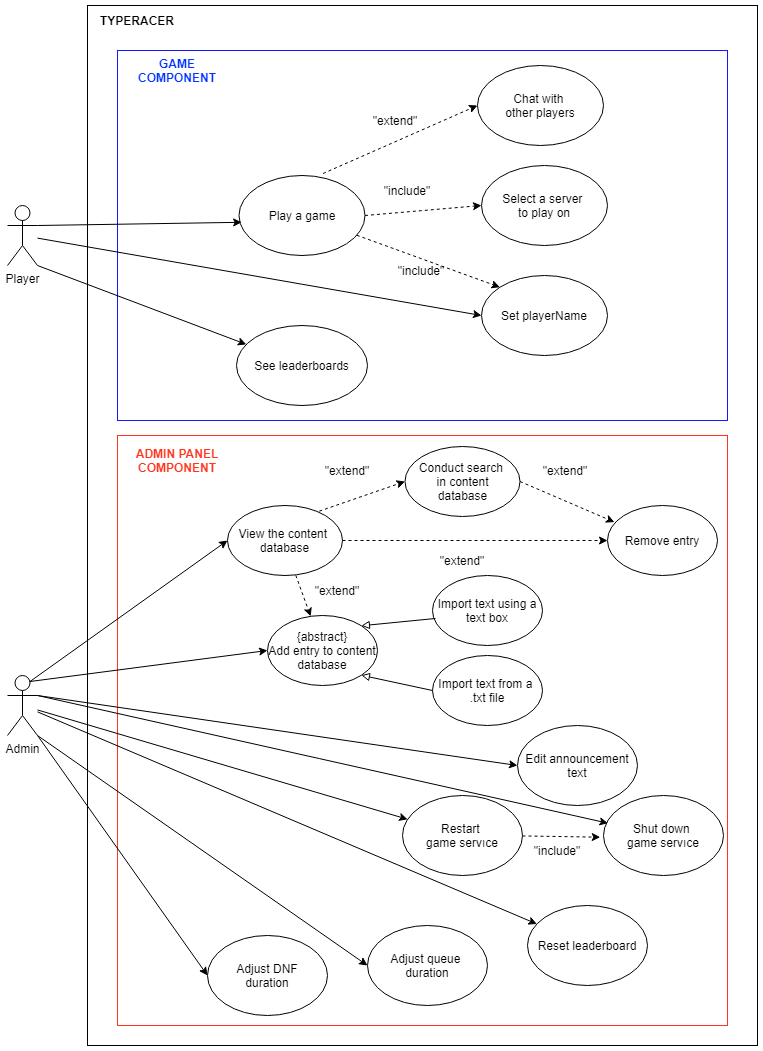
\includegraphics[width=0.85\textwidth]{TypeRacerUseCase.drawio.png}
\end{figure}

\end{document}
